\documentclass[main.tex]{subfiles}
\begin{document}


\chapter{Neutrino physics}


%\begin{flushright}
%\textit{Deep in the human unconscious \\
%is a pervasive need for a logical universe that makes sense.\\
%But the real universe is always one step beyond logic.}\\
%Frank Herbert, \textit{Dune}.
%\end{flushright}



\NI Important milestones in our understanding of the neutrino properties have been achieved these last decades. The discovery of their oscillation, rewarded in 2015 by the Nobel prize of physics, proves that neutrinos are massive particles and that the lepton flavour is not conserved which challenge the Standard Model and open questions on neutrino nature. The neutrino discovery and their history are briefly presented in Section~\ref{sec:NeutrinoHistory}. Their description in the framework of the Standard Model can be found in Section~\ref{sec:NeutrinoInSM}. The neutrino oscillation phenomenom is described in Section~\ref{sec:NeutrinoMixing}. Finally, Section~\ref{sec:MassiveNeutrino} discusses the massive neutrinos and the different methods which could give access to it.


\section{Neutrino history}\label{sec:NeutrinoHistory}


\NI The history of neutrino physics started in 1914 when J. Chadwick measured the energy spectrum of the electron emitted in $\beta$ decay~\cite{ChadwickBetaSpectrum}. At that time, this decay was considered, as the $\alpha$ and $\gamma$ decays, as the emission of a single particle and the observation of a continuous spectrum instead of a monoenergetic line go against the fundamental principe of the energy conservation. To solve this problem, W. Pauli proposed that a part of the energy is carried away by a second, electrically neutral, weakly interacting and very light particle~\cite{PauliLetter}. To distinguish this new particle from the heavier neutron, E. Amaldi called it in jest, neutrino. This name has then be widespreaded by E. Fermi during the Paris and Solvay conferences in 1932 and 1933 respectively. Twenty six years after its prediction, neutrino has finally been discovered by the Cowan and Reines experiment installed near a nuclear reactor~\cite{CowanReines}.


\bigskip


\NI In 1934, E. Fermi provided a theoretical description of the beta decay~\cite{FermiTheory} in which four fermions directly interact at a common vertex. The Fermi interaction was the precursor to the theory for the weak interaction introduced by S.~Glashow, A~Salam and S.~Weinberg~\cite{Glashow,Salam,Weinberg}. In these models, the electron and the neutrino are deeply linked since there are always created together. In 1936, the discovery of a second electron flavour, the muon $\mu$~\cite{MuonDiscovery}, suggested the existence of a second neutrino $\nu_\mu$, discovered in 1962 at Brookhaven~\cite{MuonNeutrino}. In the same way, the detection of the lepton $\tau$ in 1975~\cite{TauDiscovery} leaded to the $\nu_\tau$ discovery in 2000 by the DONUT experiment~\cite{TauNeutrino}. Nowadays, thanks to the very precise measurements of the invisible width of the Z boson\footnote{Corresponding to the channel decay Z$^\text{0} \rightarrow \nu + \bar{\nu}$} realized at CERN with the LEP collider, we know that it exists three active flavours of light neutrinos as shown in Figure~\ref{LEP-Z0-width}.



\begin{figure}
\begin{center}
\includegraphics[scale=0.4]{pictures/Chap1/Nnu.pdf}
\caption{Combined LEP cross-section measurement for e$^+$e$^-$ $\rightarrow$ hadrons around the Z$^\text{0}$ resonance. N$_{\nu}$ = 3 is clearly favoured~\cite{ALEPH3neutrino}.}
\label{LEP-Z0-width}
\end{center}
\end{figure}


\FloatBarrier


\section{Neutrino in the Standard Model}\label{sec:NeutrinoInSM}


\NI The Standard Model ($\mathcal{SM}$) is the quantum field theory describing the fundamental constituents of the Universe and the way they interact. The theory is based in the gauge group SU(3)$_\text{c}$ $\otimes$ SU(2)$_\text{L}$ $\otimes$ U(1)$_\text{Y}$ where C,L and Y denote color, left handed chirality and weak hypercharge respectively. 


\section{Neutrino mixing}\label{sec:NeutrinoMixing}


\NI In the $\mathcal{SM}$, neutrinos are massless and there is no mixing between the leptonic flavours since the mass eigenstates are degenerated. In the late of 1960s, the Homestake experiment detected for the time the neutrino emitted by the Sun and measured a deficit in the neutrino flux~\cite{Homestake}. This discrepancy between the predicted and measured rates of neutrino detection has been confirmed by other experiments such as SAGE~\cite{SAGE} or GALLEX~\cite{Gallex} and could be explained by an oscillation phenomena of the neutrino during its propagation. Another discrepancy between the predicted and measured atmospheric neutrino flux have also been observed~\cite{AtmosphericAnomaly}. 


\bigskip


\NI The neutrino oscillation hypothesis has been confirmed in 1998 by the SNO~\cite{SNO} and SuperKamiokande experiments~\cite{SK} and has been rewarded by a Nobel prize in 2015. Nowadays, the mechanism responsible of neutrino oscillation is well known and described by the theory and the experimental observations. The theoretical framework of the neutrino oscillation is introduced in Section~\ref{sec:NeutrinoOscillationTheory}. The observation status in the different sectors is summarized in Section~\ref{sec:ObservationStatusOscillation}. The open questions and the future of neutrino parameter measurements are introduced in Section~\ref{sec:SummaryOpenQuestions}.


\subsection{Neutrino oscillation}\label{sec:NeutrinoOscillationTheory}


\NI In analogy to the $\text{K}^\text{0} \leftrightarrow \bar{\text{K}}^\text{0}$ oscillation in quark sector, Pontecorvo postulated the possibility of the neutrino oscillation $\nu \leftrightarrow \bar{\nu}$ in 1957~\cite{PontecorvoOscillationProposal}. After the discovery of the $\nu_\mu$, Maki, Nakagawa and Sakata proposed the possibility of oscillation among the neutrino families~\cite{MakiNakagawaSakata}. The mechanism of the neutrino oscillation is based on the fact, in a scenario a massive neutrino, flavour states $|\nu_\alpha \rangle$ and mass states $|\nu_\text{i} \rangle$ could not coincide : 


\begin{equation}\label{eq:RelationEigenStateMassFlavor}
 |\nu_\alpha \rangle = \sum_\text{i} U_{\alpha,\text{i}}^{*} |\nu_\text{i} \rangle
\end{equation}


\NI where $\alpha$ represents the flavours (e,$\mu$,$\tau$), i enumerates the mass value of the mass state (1,2,3) and U is the PMNS (Pontecorvo-Maki-Nakagawa-Sakata) unitary matrix. The free propagation of the mass eigenstates follows the Schrödinger equation and can be described by plane wave solutions of the form : 


\begin{equation}
|\nu_\text{i} (\text{t}) \rangle = \text{e}^{-i(\text{E}_\text{i}\text{t}-\text{p}_\text{i}\text{L})} |\nu_\text{i} (\text{0}) \rangle
\end{equation}


\NI where E$_\text{i}$ is the energy of the mass eigenstate i, t is the start from the start of the propagation, p$_\text{i}$ is the momentum and L is the propagation distance. By assuming the three mass eigenstates propagate with the same momentum with relativistic energy (p $\simeq$ E > m) : 


\begin{equation}
\text{E}_\text{i} = \sqrt{\text{p}_\text{i}^\text{2} +\text{m}_\text{i}^\text{2}} \simeq \text{p} + \frac{\text{m}_\text{i}^\text{2}}{\text{2p}} \simeq \text{E} = \frac{\text{m}_\text{i}^\text{2}}{\text{2E}}
\end{equation}


\NI Equation~\ref{eq:RelationEigenStateMassFlavor} can be written, using the natural units (c = $\hbar$ = 1, ) as : 


\begin{equation}
|\nu_\alpha (\text{t}) \rangle = \sum_\text{i} \text{U}_{\alpha \text{i}}^*~\text{e}^{-i(\text{m}_\text{i}^\text{2}/\text{2E})\text{L}}~|\nu_\text{i} (\text{0}) \rangle 
\end{equation}


\NI The eigenstates propagate with different frequencies depending on their mass. By reverting Equation~\ref{eq:RelationEigenStateMassFlavor}, the mass eigenstate $|\nu_\text{i} \rangle$ can be written as a function of the flavour eigenstate $|\nu_\beta \rangle$ :  


\begin{equation}\label{eq:FlavourToFlavour}
|\nu_\alpha\rangle  = \sum_{\beta\in(e,\mu,\tau)} \left( \sum_\text{i} \text{U}_{\alpha \text{i}}^*~\text{e}^{-i(\text{m}_\text{i}^\text{2}/\text{2E})\text{L}} \text{U}_{\beta \text{i}} \right)~|\nu_\beta \rangle
\end{equation}


\NI Equation~\ref{eq:FlavourToFlavour} shows that a neutrino created with a flavour state $\alpha$ evolves as a linear superposition of the existing lepton states. The probability to observe a neutrino created with flavour $\alpha$ with a different flavour $\beta$ after a distance L is given by : 


 
\begin{equation}\label{eq:OscillationNeutrino}
\begin{split}
\text{P} (\nu_\alpha \rightarrow \nu_\beta) (\text{L},\text{E}) & = |\langle \nu_\beta|\nu_\alpha(\text{L})|^\text{2} \\[0.2cm]
 & = \sum_\text{i} |U_{\alpha\text{i}}U_{\beta\text{i}}^*|^\text{2} + 2 \mathcal{R}e \left( \sum_\text{i>j} U_{\alpha\text{i}}U_{\beta\text{i}}^*U_{\alpha\text{j}}^*U_{\beta\text{j}}~\text{e}^{-i(\Delta\text{m}_\text{ij}^\text{2}/\text{2E})\text{L}}  \right)
\end{split}
\end{equation}


\NI where $\Delta \text{m}_{\text{ij}}^\text{2} = \text{m}_\text{i}^\text{2} - \text{m}_\text{j}^\text{2}$ is the mass squared difference related via : $\Delta \text{m}_{\text{12}}^\text{2}~+~\Delta~\text{m}_{\text{23}}^\text{2}~+~\Delta \text{m}_{\text{13}}^\text{2}~=~\text{0}$. In Equation~\ref{eq:OscillationNeutrino}, an oscillation term appears as a function of the distance between the neutrino creation point and the detection point, and the neutrino energy. The oscillation frequency is proportional to $\Delta \text{m}_{\text{ij}}^\text{2}$ while the oscillation amplitude is proportional to the PMNS matrix elements U$_{\alpha\text{i}}$~:


\begin{equation}
\text{U} = \left( \begin{array}{ccc}
\text{c}_{\text{12}}~\text{c}_{\text{13}} & \text{s}_{\text{12}}~\text{c}_{\text{13}} & \text{s}_{\text{13}}~\text{e}^{-i\delta} \\
-\text{s}_{\text{12}}~\text{c}_{\text{23}} - \text{c}_{\text{12}}~\text{s}_{\text{23}}~\text{s}_{\text{13}}~\text{e}^{i\delta} & \text{c}_{\text{12}}~\text{c}_{\text{23}} - \text{s}_{\text{12}}~\text{s}_{\text{23}}~\text{c}_{\text{13}}~\text{e}^{i\delta}  & \text{s}_{\text{23}}~\text{c}_{\text{13}} \\
\text{s}_{\text{12}}~\text{s}_{\text{23}} - \text{c}_{\text{12}}~\text{c}_{\text{23}} \text{s}_{\text{13}}~\text{e}^{i\delta} & -\text{c}_{\text{12}}~\text{s}_{\text{23}} - \text{s}_{\text{12}}~\text{c}_{\text{23}}~\text{s}_{\text{13}}~\text{e}^{i\delta} & \text{c}_{\text{23}}~\text{c}_{\text{13}} \\
\end{array} \right)
\end{equation}


\NI where c$_{ij}$ = cos~$\theta_{\text{ij}}$ and s$_{ij}$ = sin~$\theta_{\text{ij}}$ with the mixing angles $\theta_{\text{12}}$, $\theta_{\text{23}}$ and $\theta_{\text{13}}$, and $\delta$ is a CP violation phase. The neutrino oscillation depends on 6 parameters : 3 mixing angles, 2 mass squared differences and a complex CP violation phase. For pratical reason, the mixing matrix is usually factorized in 3 matrices M$_{\text{23}}$ $\times$ M$_{\text{13}}$ $\times$ M$_{\text{12}}$ :  
   
   
\begin{equation}
\text{U} = \underbrace{ \left(( \begin{array}{ccc}
\text{1} & \text{0}               & \text{0} \\
\text{0} & \text{c}_{\text{23}}   & \text{s}_{\text{23}} \\
\text{0} &  -\text{s}_{\text{23}} & \text{c}_{\text{23}} \\
\end{array} \right)}_{\text{Atmospheric}}~\underbrace{ \left( \begin{array}{ccc}
\text{c}_{\text{13}}                       & \text{0} & \text{s}_{\text{13}}~\text{e}^{-i\delta} \\
\text{0}                                  & \text{1} & \text{0}  \\
-\text{s}_{\text{13}}~\text{e}^{-i\delta} & \text{0} & \text{c}_{\text{13}} \\
\end{array} \right)}_{\text{Cross}-\text{mixing}}~\underbrace{\left( \begin{array}{ccc}
\text{c}_{\text{12}}  & \text{s}_{\text{12}} & \text{0} \\
-\text{s}_{\text{12}} & \text{c}_{\text{12}} & \text{0} \\
\text{0}              & \text{0}             & \text{1} \\     
\end{array} \right)}_{\text{Solar}}
\end{equation}


\NI An additional matrix is added in case of Majorana neutrinos with two phases $\lambda_\text{1}$ and $\lambda_\text{2}$ but does not impact the neutrino oscillation :


\begin{equation}
\text{U} = \text{M}_{\text{13}} \times \text{M}_{\text{23}} \times \text{M}_{\text{12}} \times \underbrace{ \left( \begin{array}{ccc}
\text{1}                    & \text{0}                    & \text{0} \\
\text{0}                    & \text{e}^{i\lambda_\text{1}} & \text{0} \\
\text{0}                    & \text{0}                    & \text{e}^{i\lambda_\text{2}}\\
\end{array} \right) }_{\text{In case of Majorana neutrino}}  
\end{equation} 


\NI The matrix M$_{\text{23}}$ is parametrized in term of $\theta_{\text{23}}$ which is the mixing angle dominating the $\nu_\mu \rightarrow \nu_\tau$ and related to the atmospheric neutrino. The matrix M$_{\text{12}}$ is parametrized in term of $\theta_{\text{12}}$ which is the mixing angle dominating the $\nu_\text{e} \rightarrow \nu_{\mu,\tau}$ and related to the solar neutrinos. The matrix M$_{\text{13}}$ is parametrized in term of $\theta_{\text{13}}$ which is the mixing angle dominating the $\nu_\mu \rightarrow \nu_\text{e}$


\FloatBarrier


\subsection{Observation status}\label{sec:ObservationStatusOscillation}


\NI In order to easily understand the neutrino oscillation experimental results, we consider the case with only two active neutrinos. This case is equivalent to consider that only one squared mass splitting $\Delta$m$_\text{ij}^\text{2}$ is important compared to the others. This approximation is possible because two of the mass splitting are very close compared to the third and the mixing angle $\theta_\text{13}$ is small. This case is appropriate for the case of atmospheric neutrinos mixing ($\nu_\mu \rightarrow \nu_\tau$) where the $\nu_e$ plays no role and also for the solar case and for short baseline reactor antineutrino experiment. Considering two flavour states $\nu_\alpha$ and $\nu_\beta$, two mass states $\nu_\text{1}$ and $\nu_\text{2}$ and their difference mass splitting $\Delta$m$^\text{2}$ = m$_\text{2}^\text{2}$ - m$_\text{1}^\text{2}$. The mixing among the neutrino families is described a unitary 2$\times$2 matrix : 


\begin{equation}
\left( \begin{array}{c}
\nu_\alpha \\
\nu_\beta
\end{array} \right) = \left(  \begin{array}{cc}
\text{cos}~\theta & \text{sin}~\theta \\
-\text{sin}~\theta & \text{cos}~\theta \\
\end{array}
\right) \left( \begin{array}{c}
\nu_\text{i} \\
\nu_\text{j} \\
\end{array} \right)
\end{equation}


\smallskip


\NI where $\theta$ is the rotation angle between the flavour and the mass eigenstate. The oscillation probability is then written :  


\begin{equation}
\text{P}_{\nu_\alpha \rightarrow \nu_\beta} (\text{L},\text{E}) = \text{sin}^\text{2}(\text{2}\theta)~\text{sin}^\text{2} \left( \frac{\Delta \text{m}^\text{2} \text{L}}{\text{4E}} \right)
\end{equation}


\NI this last expression can also be written using the physics units : 


\begin{equation}
\text{P}_{\nu_\alpha \rightarrow \nu_\beta} (\text{L},\text{E}) = \text{sin}^\text{2}(\text{2}\theta)~\text{sin}^\text{2} \underbrace{\left(  \text{1.27}~\Delta \text{m}^\text{2} [\text{eV}^\text{2}] \frac{\text{L}[\text{km}]}{\text{4E}[\text{GeV}]} \right)}_\phi
\end{equation}


\NI In the limit where $\phi$ $<<$ 1, the oscillation probability can be approximated to : 


\begin{equation}
\text{P}_{\nu_\alpha \rightarrow \nu_\beta} (\text{L},\text{E}) \simeq \text{sin}^\text{2} \text{2}\theta  \left( \frac{\Delta\text{m}^\text{2}\text{L}}{\text{4E}} \right)^\text{2} 
\end{equation}


\NI and the measurement of the oscillation probability would give information on the product sin$^\text{2}$(2$\theta$)~$\times$~$\Delta$m$^\text{2}$. Given L/E, neutrino oscillation experiments then provide two parameters : the oscillation frequency $\Delta$m$^\text{2}$ and the mixing angle $\theta$. Depending on the sector they are sensitive, oscillation neutrino experiment are classified in solar, atmospheric, reactor and accelerator experiments. 


\subsubsection{Solar neutrino}


\NI The Sun produces an important flux of electron neutrinos during the thermonuclear fusion process, 6.10$^{\text{10}}$ neutrinos/cm$^{\text{2}}$/s arrive at the surface of the Earth. The typical energy of the solar neutrino is at the order of 1~MeV. In the 1970s, the first observation of these neutrinos was realised by the Homestake experiment~\cite{Homestake}. The experiment points out a deficit of neutrinos comparing with the standard solar model prediction~\cite{NeutrinoFluxSolar}, only one third were measured. This deficit has been confirmed by other experiments such as Gallex, SAGE or Kamiokande~\cite{Gallex,SAGE,Kamiokande2} and was known as the solar neutrino problem. In 2001, the SNO experiment (Sudbury Neutrino Observatory) used an heavy water detector allowing the detection of the three neutrino flavours and proved that the deficit is consistent with a neutrinos flavour mixing~\cite{SNO}.


\bigskip


\NI The solar neutrinos have also been studied by the KamLAND experiment located in the Kamioka mine in Japan~\cite{Kamiokande2}. KamLAND showed that to explain all the neutrino deficit of solar neutrino, the oscillation in vacuum is not enough and that there is an important effects of neutrino oscillation in matter called MSW effect~\cite{MSW}. Combining KamLAND results with different solar experiments, the actual values of the parameters in the solar sector have been determined~\cite{PDG2016} : 

   

\begin{gather}
\Delta\text{m}_{\text{21}}^{\text{2}} = \text{7.53} \pm \text{0.18} \times \text{10}^{\text{\text{-5}}}~~\text{eV}^\text{2} \nonumber\\[1.5ex]
\text{sin}^\text{2} \theta_{\text{12}} = \text{0.307} \pm \text{0.013} 
\end{gather}


%\begin{figure}
%\begin{center}
%\includegraphics[scale=0.65]{pictures/Chap1/SNO.pdf}
%\caption{a}
%\end{center}
%\end{figure}


\FloatBarrier


\subsubsection{Atmospheric neutrino}

\NI The interaction of cosmic rays with the atmosphere of the Earth can produce hadronic showers containing pions and kaons. The decays of these particles creates high energy muons and muon neutrino. Muons at low energy (< 1~MeV) decay before hitting the Earth's surface into electron, $\nu_e$ and $\nu_\mu$~: 


\begin{gather}
\pi^{\pm} \rightarrow \mu^{\pm} + \nu_\mu~(\bar{\nu_\mu})
\nonumber\\[1.5ex]
\mu^\pm \rightarrow e^\pm + \nu_e~(\bar{\nu_e}) + \nu_\mu~(\bar{\nu_\mu})  
\end{gather}


\NI At these energies, we expected to detect twice more $\nu_\mu$~($\bar{\nu_\mu}$) than $\nu_e$~($\bar{\nu_e}$)~\cite{AtmosNeutrinoFlux}. Some experiments measured a deficit of $\nu_\mu$ giving origin to the so called atmospheric neutrino anomaly~\cite{AtmosNeutrinoAnomaly}. Several interpretations have been proposed to solved this anomaly such as Lorentz invariance violation, flavor changing neutral currents or neutrino oscillations. In 1998, the SuperKamiokande experiment, successor of the Kamiokande detector, confirmed the deficit and demonstrated its dependance depending on the zenital angle as shown in Figure~\ref{SKzenitalDependance}. In an underground detector as SuperKamiokande the flux of neutrinos going up is expected to be the same as the neutrino going down because the neutrino flux produced in the atmosphere is expected to be isotropic. In Figure~\ref{SKzenitalDependance}, sub-GeV $\nu_e$ have almost no dependance on the zenith angle while the flux of going down $\nu_\mu$ is higher than the up going neutrino at sub-GeV scale. These results can be interpreted in term of oscillations : $\nu_\mu$ going down are produced at opposite side of the Earth and travelled around 12~000~km more than the $\nu_\mu$ going down. It seems than these going down $\nu_\mu$ disappear during their propagation while no disappearence of $\nu_e$ has been found. This is interpreted as an oscillation of the $\nu_\mu$ into $\nu_\tau$~\cite{EvidenceAtmosNeutrinoOsc}.   


%\NI SK
%\NI SK~\cite{SK}


\begin{figure}
\begin{center}
\includegraphics[scale=0.4]{pictures/Chap1/sk.png}
\caption{Angular distributions of the electron and muon neutrinos produced in the atmosphere measured by SuperKamiokande. The $\nu_\mu$ neutrino rate presents a clear deficit for the neutrinos crossing the Earth (cos $\theta$ < 0) compared to the predicted flux without no oscillation (red~line)~\cite{SK}.}
\label{SKzenitalDependance}
\end{center}
\end{figure}


\bigskip


\NI The hypothesis of neutrino oscillation $\nu_\mu \rightarrow \nu_\tau$ have been confirmed by disappearance experiment measurements such as K2K or MINOS~\cite{K2K,MINOS}. These experiments studied the $\nu_\mu$ flux created by an accelerator with a near and a far detector. The near detector allow the measurement of the $\nu_\mu$ flux going to the far detector. With the knowledge of their energy and the distance between the near and far detector, the oscillation parameters can be extracted. To definitely confirm the $\nu_\mu \rightarrow \nu_\tau$ oscillation, the OPERA experiment searched and found the $\nu_\tau$ apparence in a pure $\nu_\mu$ beam~\cite{Opera}. Combining the atmospheric with the reactor data, the global fit concerning the parameters in the atmospheric sector have been determined to be : 


\begin{gather}
\Delta\text{m}_{\text{23}}^{\text{2}} = \text{2.45} \pm \text{0.05} \times \text{10}^{\text{\text{-3}}} \text{eV}^\text{2}
\nonumber\\[1.5ex]
\text{sin}^\text{2} \theta_{\text{23}} = \text{0.51} \pm \text{0.04} 
\end{gather} 




\FloatBarrier


\subsubsection{Reactor neutrino}


\NI Nuclear reactors are a very intense source of neutrino. An important part of elements created during the uranium fission decay by $\beta$ decay leading to a continous $\bar{\nu}_e$ flux with an energy of the order of MeV. A 1 GW reactor emits around 10$^\text{20}$ neutrinos/s. 


\bigskip


\NI The $\bar{\nu}_e$ oscillation to $\bar{\nu}_\mu$ and $\bar{\nu}_\tau$ can only be measured by the disappearance of the $\bar{\nu}_e$ since the energy is not high enough for the $\mu$ and $\tau$ creation. Generally the detection of the $\bar{\nu}_e$ is realized by inverse beta decay reaction ($\bar{\nu}_e$ + p $\rightarrow$ n + e$^+$). The coincidence detection of the photons emitted by the positron annihilation and by the neutron capture allows to identify the $\bar{\nu}_e$ interaction in the detector. The first detection of the neutrino in 1956 used with technique which is still used today such as in the KamLAND and the DayaBay experiments~\cite{KamLAND,DayaBay}. Figure~\ref{sec:ReactorNeutrinoExperiment} shows the oscillation survival probability versus L$_\text{eff}$/E$_\nu$.


\begin{figure}
\begin{center}
\includegraphics[scale=0.4]{pictures/Chap1/KAMLAND.pdf}
\includegraphics[scale=0.5]{pictures/Chap1/osc_loe_NL2015.pdf}
\caption{Measured reactor $\bar{\nu}_e$ spectral distortion displayed as the oscillation survival probability versus L$_\text{eff}$/E$_\nu$. Top : results from KamLAND~\cite{KamLAND}. Bottom : results from DayaBay~\cite{DayaBay}.}
\label{sec:ReactorNeutrinoExperiment}
\end{center}
\end{figure}


\NI These baseline experiments allow the measurement of the $\Delta$m$^\text{2}_\text{13}$ and $\theta_\text{13}$ parameters. Moreover the $\Delta$m$^\text{2}_\text{13}$ parameter can be constrained from atmospheric and accelerator neutrino experiments. The global fit gives :  


\begin{gather}
\Delta\text{m}_{\text{13}}^{\text{2}} = \text{2.45} \pm \text{0.05} \times \text{10}^{\text{\text{-3}}} \text{eV}^\text{2}
\nonumber\\[1.5ex]
\text{sin}^\text{2} \theta_{\text{13}} = \text{0.021} \pm \text{0.0011} 
\end{gather} 


\FloatBarrier


\subsubsection{Accelerator neutrino}


\NI Today particle accelerators can be used as source of artificial neutrino, mainly $\nu_\mu$. The advantage is that the characteristics of the neutrino beam are well known and can be adapted (energy and $\nu$/$\bar{\nu}$). To create the $\nu_\mu$ (or $\bar{\nu}_\mu$) beam, the principle is to send a proton beam on a target to produce hadrons (pions, kaons,...) which then decay mainly into $\mu$ and $\nu_\mu$. A detector is placed hundred kilometers away to measure the $\nu_\mu$ disappearance or the $\nu_{e,\tau}$ appearance. It has existed and there are still many neutrino accelerator experiments around the world such as MiniBooNE, MINOS, T2K or No$\nu$A. I will not discuss all of them here, their physics program are very wide including the measurement of the mixing angle $\theta_\text{13}$, the determination of the CP-violating phase, mass ordering or search for sterile neutrinos. One of these experiment, OPERA, found 5 $\nu_\tau$ events, after 5 years of data taking confirming the $\nu_\mu \rightarrow \nu_\tau$ oscillation~\cite{Opera,OperaTau}.


%\NI T2K, ~\cite{T2Knim,T2KNue2nd,T2Knumu2nd}


\FloatBarrier


\subsection{Summary and open questions}\label{sec:SummaryOpenQuestions}


\NI The neutrino oscillation phenomenom has been studied by many experiments and is fairly well understood by the theory and experience. The measurement of the three mixing angles are more and more precise and are known today with a precision less than~10\%. The two squarred mass splitting have been also been measured. Future neutrino experiments will focus on the determination of the missing oscillation parameter $\delta_\text{CP}$ and of the sign of the $\Delta\text{m}^\text{2}_\text{31}$. Others experiments also investigate the possibility of the existence of sterile neutrinos.


%The last update measurements are summarised in Table~\ref{}.
%\begin{table}
%\centering
%\begin{tabular}{c|c}
%\toprule
%Oscillation parameter & Values  \\[0.1cm]
%\hline
%sin$^\text{2}$ $\theta_{\text{12}}$ & 0.307 $\pm$ 0.013                            \\[0.1cm]
%sin$^\text{2}$ $\theta_{\text{13}}$ & (2.10 $\pm$ 0.11) $\times$ 10$^{-\text{2}}$  \\[0.1cm]
%sin$^\text{2}$ $\theta_{\text{23}}$ & 0.51 $\pm$ 0.04  (0.50 $\pm$ 0.04)           \\[0.1cm]
%$\Delta$m$_{\text{12}}^\text{2}$    & (7.53 $\pm$ 0.18) $\times$ 10$^{-\text{5}}$ eV$^\text{2}$ \\[0.1cm]
%$\Delta$m$_{\text{23}}^\text{2}$    & 2.45 $\pm$ 0.05 $\times$ 10$^{-\text{3}}$ eV$^\text{2}$  (2.52 $\pm$ 0.05 $\times$ 10$^{-\text{3}}$ eV$^\text{2}$) \\[0.1cm]
%\bottomrule
%\end{tabular}
%\caption{aa}
%\label{tab:zzz}
%\end{table} 

\subsubsection{CP violation phase}


\NI The last oscillation parameter which has not still be measured yet is the CP violating phase $\delta_\text{CP}$. The measurement of this parameter is motivated since it can demonstrate difference in the behaviour between the neutrino and antineutrino which could explain the mater/antimatter asymmetry in the Universe. The future long baseline experiments such as DUNE or HyperKamiokande will determine this parameter in the next 10 years~\cite{DUNE,HK}. 


\subsubsection{Mass ordering}


\NI Neutrino oscillations provide information on the mass squared differences and do not allow to access to their mass. Thanks to solar neutrino measurements $\Delta\text{m}^\text{2}_\text{21}$ have been determined to be positive but we still do not know the sign of $\Delta\text{m}^\text{2}_\text{31}$. Two cases are then possible as shown in Figure~\ref{MassOrdering}, if $\Delta\text{m}^\text{2}_\text{31}$ > 0 we talk about normal ordering, if $\Delta\text{m}^\text{2}_\text{31}$ < 0 we talk about inverted hierarchy. Some experiments are planned in the future to determine the neutrino mass ordering such as JUNO, PINGU or KM3NeT~\cite{JUNO,PINGU,KM3NeT}. The determination of the neutrino mass ordering is important since it strongly impact the neutrinoless double beta decay researches and the measurements of $\delta_\text{CP}$.


\begin{figure}
\begin{center}
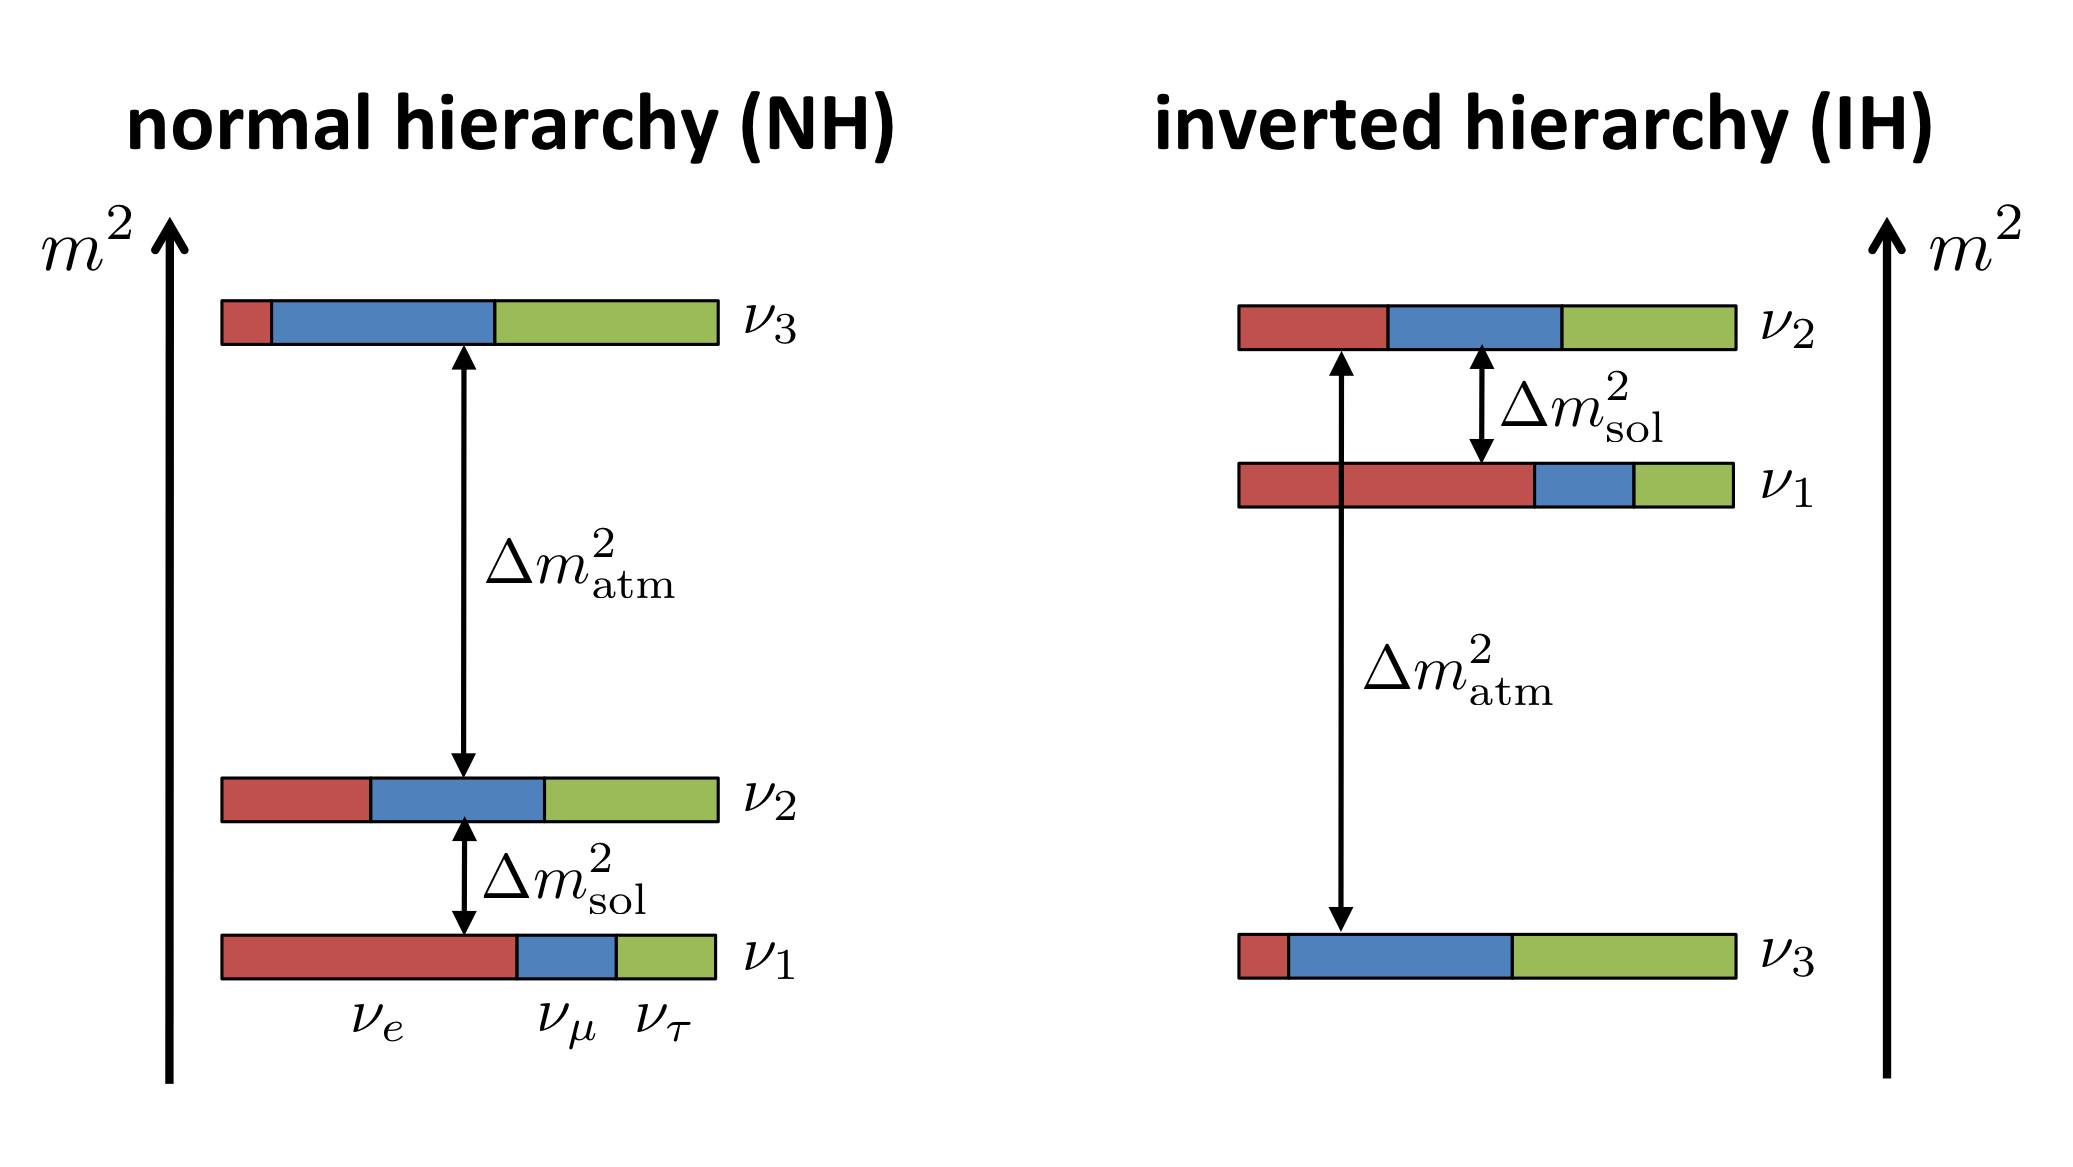
\includegraphics[scale=0.13]{pictures/Chap1/mass-hierarchy.png}
\caption{Neutrino mass ordering : on the left the normal ordering where $\Delta\text{m}^\text{2}_\text{31}$ > 0. On the right the inverted ordering where $\Delta\text{m}^\text{2}_\text{31}$ < 0.}
\label{MassOrdering}
\end{center}
\end{figure}


\FloatBarrier


\subsubsection{Sterile neutrino}


\NI Despite the success of the three flavour oscillation theory, some small anomalies in short baseline neutrino experiments have been highlighted which can not be explained in the three neutrino framework. These anomalies could suggest that the theory is incomplete and could point out the existence of sterile neutrino.


\bigskip


\NI During the development of the last generation of reactor neutrino experiments, the $\bar{\nu}_e$ flux have been reevaluated~\cite{PredictionReactorAntiNeutrino1,PredictionReactorAntiNeutrino2}. A total deficit of approximately 7\% have been found between the updated predicted flux and the flux measured by different experiments~\cite{DeficitReactor7}. This discrepency is called the reactor antineutrino anomaly~\cite{ReactorAnomaly}. 


\bigskip


\NI Another anomaly have been measured by the GALLEX~\cite{Gallex} and SAGE~\cite{SAGE} experiments. These experiments were calibrated with $^{\text{51}}$Cr and $^{\text{37}}$Ar sources places inside the detector. The monoenergetic $\nu_e$ produced by these sources was detected by their interaction with $^{\text{71}}$Ga forming $^{\text{71}}$Ge. A deficit between the measured and the predicted event rates have been found corresponding to a 2.8~$\sigma$ deviation~\cite{LightSterileNeutrino}. This anomaly is called gallium anomaly.


\bigskip


\NI In addition to these two anomalies a last one coming from the LSND experiment have been highlighted. This experiment measured an excess of 3.8~$\sigma$ of $\bar{\nu}_e$ events in a beam of $\nu_\mu$ produced by $\mu$ decays~\cite{LSND}. To explain all these anomalies, the existence of a sterile neutrino have been postulated. The best fit values for the oscillation parameters suggest $\Delta$m$^\text{2}$~>~1.5~eV$^\text{2}$ and sin$^\text{2}$2$\theta$~=~0.14~$\pm$~0.08~\cite{ReactorAnomaly}. Experiments are currently running or building to exclude or confirm the existence of a light sterile neutrino such as STEREO~\cite{STERO}, Solid~\cite{Solid} or SOX~\cite{SOX}. First results should arrive in the coming months.


\FloatBarrier


\section{Massive neutrino}\label{sec:MassiveNeutrino}

\NI The observation of neutrino oscillations proves that neutrinos are massive particles which is in direct conflict with their description in the current form of the $\mathcal{SM}$. The origin of their mass is believed as a low energy manifestation of physics behond $\mathcal{SM}$. Section~\ref{sec:OriginNeutrinoMass} describes the mechanisms which can give a mass to the neutrino while Section~\ref{sec:NeutrinoMassMeasurementExp} discusses the different ways which could allow us to measure it.


\subsection{Origin of neutrino mass}\label{sec:OriginNeutrinoMass}


\NI The origin of the neutrino mass has been subject to an intense theoretical and experimental investigations. To introduce the neutrino into the $\mathcal{SM}$, two different types of neutrino mass terms are possible : Dirac and Majorana.

\subsubsection{Dirac term mass}


\NI A straightforward way to generate a neutrino mass is to use the same Higgs mechanism that gives mass to quarks and charged leptons. In this scenario, the existence of a right handed neutrino has to be postulated. To agree with experimental observations, these right handed neutrinos can not couple to the weak interaction and are called sterile~\cite{DiracNeutrino}. The Dirac mass term is written as : 


\begin{equation}\label{eq:DiracMassTerm}
\mathcal{L}_{\text{mass}}^\text{D} = -\text{m}_\text{D} ( \overline{\nu_\text{R}}~\nu_\text{L} + \overline{\nu_\text{L}}~\nu_\text{R} ) 
\end{equation}


\smallskip


\NI where $\nu_{\text{R}}$ and $\nu_{\text{L}}$ are the right and left handed chiral fields for the neutrino and m$_\text{D}$ is the Dirac mass matrix which can be expressed for the componant k in term of the Yukawa coupling $\lambda_\text{k}^{\nu}$ and  the vacuum expectation value $v$ : 

\begin{equation}
\text{m}_\text{k} = \frac{\lambda_\text{k}^\nu v}{\sqrt{\text{2}}}
\end{equation}  


\smallskip


\NI Dirac neutrino acquire their mass by coupling to the Higgs field and their mass are proportional to $v$. The main problem of this mechanism is that it does not explained the huge order of magnitude difference between the charged lepton and neutrino masses. There are four distinct fields in Equation~\ref{eq:DiracMassTerm} which implies that neutrino and anti-neutrinos are fundamentally different particles.


\subsubsection{Majorana term mass}

\NI Another way to introduce a mass term into the $\mathcal{SM}$ is through a Majorana mass term. This term have been proposed for the first time in 1937 by Ettore Majorana~\cite{Majorana2008}. It consists of introducing a Majorana field defined such that $\mathcal{C}|\psi\rangle$ = $|\psi\rangle$ implying there is no distinction between particle and anti-particle. This type of mass term is only possible for electrically neutral particles such as neutrinos. For a fermion field ($\psi = \psi_\text{L} + \psi_\text{R}$), the Dirac equation ($i\gamma^\mu\partial_\mu$)$\psi = 0$ is equivalent to the coupled equations~\cite{WeylSpinorNeutrino} : 


\begin{gather}\label{eq:DiracEquations}
i\gamma^\mu\partial_\mu \psi_\text{L} = \text{m} \psi_\text{R} \nonumber\\[1.0ex]
i\gamma^\mu\partial_\mu \psi_\text{R} = \text{m} \psi_\text{L}
\end{gather}


\NI The equations are coupled by their mass term, but in case of massless field : 


\begin{gather}
i\gamma^\mu\partial_\mu \psi_\text{L} = \text{0} \nonumber\\[1.0ex]
i\gamma^\mu\partial_\mu \psi_\text{R} = \text{0}
\end{gather}


\NI the equations are not coupled and we have the so-called Weyl equations with $\psi_\text{L}$ and $\psi_\text{R}$ the Weyl spinors. As discussed in Section~\ref{sec:NeutrinoInSM}, the neutrino in the $\mathcal{SM}$ was massless and then was described by left handed Weyl spinor $\nu_\text{L}$. Majorana wondered if it is possible to make a right handed field from a left handed one to form a mass term~\cite{Majorana2008}. In the case Majorana studied, we want obtain the first equation of \ref{eq:DiracEquations} from the second one. In order to do that, the Hermitian conjugate of the second equation is taken : 


\begin{equation}\label{eq:hermitian}
-i\partial_\mu \overline{\psi_\text{R}} = \text{m} \overline{\psi_\text{L}} 
\end{equation}   
 

\NI Then the transverse of the Equation~\ref{eq:hermitian} is taken and using the property of the charge conjugaison matrix $\mathcal{C}\gamma^{\mu\text{T}} = -\gamma^\mu \mathcal{C}$ : 


\begin{equation}\label{eq:transverse}
i\gamma^\mu\partial_\mu\mathcal{C}\overline{\psi_\text{R}}^\text{T} = \text{m} \mathcal{C}\overline{\psi_L}^\text{T}
\end{equation}


\NI Equation~\ref{eq:transverse} has the same structure than the first equation of~\ref{eq:DiracEquations}, and they are identical if : 


\begin{equation}\label{eq:MajoranaRelation}
\psi_\text{R} = \xi \mathcal{C} \overline{\psi_\text{L}}^\text{T}
\end{equation}


\NI with $\xi$ is an arbitrary phase factor. Equation~\ref{eq:MajoranaRelation} is the Majorana relation between the $\psi_\text{L}$ and $\psi_\text{R}$. The Dirac equation can then be written only in terms of $\psi_\text{L}$ :


\begin{equation}
\psi = \psi_\text{L} + \psi_\text{R} = \psi_\text{L} +  \mathcal{C} \overline{\psi_\text{L}}^\text{T}
\end{equation}  


\NI implying : 


\begin{equation}\label{eq:MajoranaCondition}
\psi^\mathcal{C} = (\psi_\text{L} +  \mathcal{C} \overline{\psi_\text{L}}^\text{T})^\mathcal{C} = \psi
\end{equation}


\NI Equation~\ref{eq:MajoranaCondition} is called the Majorana condition and implies that a Majorana particle is its own antiparticle. This condition can only be satisfied by a neutral particle since the charge conjugaison opertor flips the sign of the electric charge. The only fermions that can be Majorana particles are neutrinos. In case of Majorana neutrino, the term mass is written as :  


\begin{equation}
\mathcal{L}_{\text{mass}}^\text{M} = - \frac{\text{1}}{\text{2}} \text{m}_\nu^{\text{M}} \overline{\nu_\text{L}^{\mathcal{C}}}~\nu_\text{L} + h.c
\end{equation}


\NI As Majorana mass term couples neutrinos to antineutrinos, interactions involving Majorana neutrino violate lepton number conservation by two units.


%\begin{equation}
%\psi = \psi_\text{L} + (\psi_\text{L})^\mathcal{C} ~~~ \text{and} ~~~ \psi = \psi^\mathcal{C} 
%\end{equation}


\subsubsection{See-saw mechanism}


\NI The see-saw mechanism requires Majorana neutrino. Based on the Majorana description given in Equation~\ref{eq:MajoranaCondition}, two independant fields, which are their own conjugate, can be introduced~\cite{SchechterValle,SeeSawMechanism} : 


\begin{equation}\label{eq:DefinitionSeftConjugateField}
\lambda = \frac{\chi_\text{L} + (\chi_\text{L})^\mathcal{C}}{\sqrt{\text{2}}} ~~~~~~ \Lambda = \frac{\chi_\text{R} + (\chi_\text{R})^\mathcal{C}}{\sqrt{\text{2}}}
\end{equation}


\NI The mass term in the Lagrangian can be written in its more general form : 


\begin{equation}
-\mathcal{L}_\text{m} = \text{m}_\text{L} \bar{\lambda} \lambda + \text{m}_\text{R} \bar{\Lambda} \Lambda + \text{m}_\text{D} (\bar{\lambda} \Lambda + \lambda \bar{\Lambda})
\end{equation}


\smallskip


\NI which can also be written in a matrix form as follows : 



\begin{equation}
\begin{split}
-\mathcal{L}_\text{m} = (\bar{\lambda}~\bar{\Lambda}) ~ \mathcal{M} ~ \left( \begin{array}{c} 
\lambda \\
\Lambda  
\end{array} \right) & ~~~,~~~\mathcal{M} = \left( \begin{array}{cc}
\text{m}_\text{L} & \text{m}_\text{D}^\text{T} \\
\text{m}_\text{D} & \text{m}_\text{R}
\end{array}  \right)
\end{split} 
\end{equation}


\smallskip


\NI The fields $\lambda$ and $\Lambda$ defined in Equation~\ref{eq:DefinitionSeftConjugateField} do not have a definite mass because of the non diagonal $m_\text{D}$ terms in the mass matrix. These fields are notmass eigenstates and are not physical particles. If we have mass eigenstates $\nu_\text{1}$ and $\nu_\text{2}$, the Lagrangian can be written in terms of these mass eigenstates. The $\mathcal{M}$ matrix can be diagonalized by using an unitarity matrix $\mathcal{U}$ : 


\begin{equation}
\begin{split}
\mathcal{U}^\dag \mathcal{M}~\mathcal{U} = \mathcal{M}'    & ~~~,~~~\mathcal{M}' \left(   \begin{array}{cc}
\text{m}_\text{1} & \text{0} \\
\text{0} & \text{m}_\text{2} 
\end{array} \right)
\end{split} 
\end{equation}  


\smallskip


\NI where the masses m$_\text{1}$ and m$_\text{2}$ can be expressed in terms of m$_\text{D}$, m$_\text{L}$ and m$_\text{R}$~:   


\begin{equation}
\text{m}_{\text{1,2}} = \frac{\text{1}}{\text{2}} \left[ (\text{m}_\text{L} + \text{m}_\text{R}) \pm \sqrt{(\text{m}_\text{L} - \text{m}_\text{R})^\text{2} + \text{4m}_\text{D}^\text{2}}  \right] 
\end{equation}


\smallskip


\NI As the $\mathcal{SM}$ forbids the left handed Majorana term, the mass m$_\text{L}$ can be set to 0. With this choice and making the assumption that m$_\text{R}$ $>>$ m$_\text{D}$ : 


\begin{equation}
\text{m}_{\text{1,2}} = \frac{\text{m}_\text{R}}{\text{2}} \left[\text{1} \pm \sqrt{\text{1} + \text{4} \frac{\text{m}_\text{D}^\text{2}}{\text{m}_\text{R}^\text{2}}} \right] \simeq \left\{ \begin{array}{cc}
\text{m}_\text{R} & \text{for heavy neutrino} \\
- \text{m}_\text{D}^\text{2} / \text{m}_\text{R} & \text{for light neutrino}
\end{array} \right.
\end{equation}


\smallskip


\NI The see-saw mechanism has the advantage to naturally explain the tiny mass of active neutrinos. Indeed, as the mass of the right neutrino is not constrained, an very heavy right handed neutrino can be considered leading to a very small mass for the neutrino.


\FloatBarrier


\subsection{Mass measurement}\label{sec:NeutrinoMassMeasurementExp}


\NI mini-introduction

\subsubsection{Direct neutrino mass from $\beta$ decay}


\subsubsection{Cosmology}


\newpage


\clearpage











































\begin{table}[h!]
\centering
\begin{tabular}{c|c|c|c}
\toprule
 & Particle & Charge & Mass [MeV/c$^\text{2}$] \\ [0.1cm]
\hline
\multirow{6}{*}{Quarks} & up (u)      & +2/3 & 2.2$^{+\text{0.6}}_{-\text{0.4}}$       \\ [0.1cm]
                        & down (d)    & -1/3 & 4.7$^{+\text{0.5}}_{-\text{0.4}}$       \\ [0.1cm]
                        & charm (c)   & -1/3 & (1.28 $\pm$ 0.3) $\times$ 10$^\text{3}$ \\ [0.1cm]
                        & strange (s) & +2/3 & 96$^{+\text{8}}_{-\text{4}}$            \\ [0.1cm]
                        & top (t)     & +2/3 & (160.0 - 174.2) $\times$ 10$^\text{3}$  \\ [0.1cm]
                        & bottom (b)  & -1/3 & (4.18 - 4.66) $\times$ 10$^\text{3}$    \\ [0.1cm]
\hline
\multirow{6}{*}{Leptons} & electron (e$^-$)                     & -1 & 0.5109989461 $\pm$ 0000000031 \\ [0.1cm]
                         & muon ($\mu^-$)                       & -1 & 105.6583745 $\pm$ 0.0000024   \\ [0.1cm]
                         & tau ($\tau^-$)                       & -1 & 1776.86 $\pm$ 0.12            \\ [0.1cm]
                         & electron neutrino ($\nu_{\text{e}}$) & 0  & < 2 $\times$ 10$^-\text{6}$   \\ [0.1cm]
                         & muon neutrino ($\nu_\mu$)            & 0  & < 2 $\times$ 10$^-\text{6}$   \\ [0.1cm]
                         & tau neutrino ($\nu_\tau$)            & 0  & < 2 $\times$ 10$^-\text{6}$   \\ [0.1cm]
\bottomrule
\end{tabular}
\caption{The fermion within the Standard Model of particle physics. The range of the values for the bottom and top quarks reflect the central values corresponding to differents used to extract these masses~\cite{PDG2016}.}
\label{tab:fermionSM}
\end{table}

\FloatBarrier


\begin{table}[h!]
\centering
\begin{tabular}{c|c|c|c|c}
\toprule 
Particle & Associated interaction & Spin & Charge & Mass [GeV] \\  [0.1cm]
\hline 
8 Gluons (g)           & Strong                & 1 & 0       & 0 \\  [0.1cm]
Photon ($\gamma$)      & Electromagnetic       & 1 & 0       & 0 \\  [0.1cm]
Z boson (Z$^\text{0}$) & \multirow{2}{*}{Weak} & 1 & 0       & 91.1876 $\pm$ 0.0021 \\  [0.1cm]
W boson (W$^\pm$)      &                       & 1 & $\pm$ 1 & 80.385 $\pm$ 0.015   \\  [0.1cm] 
\hline 
Higgs boson (H$^\text{0}$) & - & 0 & 0 & 125.09 $\pm$ 0.24 \\  [0.1cm]
\bottomrule 
\end{tabular} 
\caption{The bosons within the Standard Model~\cite{PDG2016}.}
\label{tab:BosonSM}
\end{table}





%\begin{figure}
%\begin{center}
%\includegraphics[scale=0.75]{/home/lenoblet-local/Bureau/Thesis/pictures/Chap1/ParticleMass_v3.pdf}
%\caption{Mass of the elementary particles. THe values are taken from~\cite{PDG2016}}
%\end{center}
%\end{figure}


%\begin{figure}[h!]
%\begin{center}
%\includegraphics[scale=1.2]{pictures/Chap1/SpectrumKatrin.jpg}
%\caption{Mass of the elementary particles. THe values are taken from~\cite{PDG2016}}
%\end{center}
%\end{figure}

%\begin{figure}
%\begin{center}
%\includegraphics[scale=0.5]{pictures/Chap1/KAMLAND.pdf}
%\caption{Combined LEP cross-section measurement for e$^+$e$^-$ $\rightarrow$ hadrons around the Z$^\text{0}$ resonance. N$_{\nu}$ = 3 is clearly favoured~\cite{KamLAND}.}
%\end{center}
%\end{figure}



KATRIN~\cite{KATRIN}
PSI\cite{PSI}
ALEPH \cite{ALEPHneutrinoTau}
Planck ~\cite{PlankNeutrinoMass}






\end{document}
